\chapter*{Lab 1 - Curve di Bézier}

I punti dell'esercitazioni che verranno trattati in questa relazione sono i seguenti:
	
\begin{itemize}
  \item Sostituire alle routine di OpenGL il disegno della curva mediante algoritmo di De Casteljau.
  \item Integrare nel programma in alternativa uno dei seguenti punti:
 	\begin{itemize}
  		\item disegno di una curva di Bézier mediante algoritmo ottimizzato basato sulla suddivisione adattiva.
  		\item disegno interattivo di una curva di Bézier composta da tratti cubici, dove ogni tratto viene raccordato con il successivo con continuità $C_0$, $C_1$, o $G_1$ a seconda della scelta utente da keyboard.
		\end{itemize}
	\item Permettere la modifica della posizione dei punti di controllo tramite trascinamento con il mouse.
\end{itemize}

\section{Struttura}
\subsection{Scenari}
L'ultimo punto è stato implementato insieme agli altri due punti.
Nel secondo punto si è scelto di implementare entrambi gli scenari. L'applicativo è quindi composto da 3 scenari selezionabili tramite la pressione dei tasti 1,2,3 dalla tastiera: 
\begin{itemize}
  \item Disegno di una curva di Bézier con algoritmo di De Casteljau
  \item Disegno di una curva di Bézier con suddivisione adattiva
  \item Disegno interattivo di più curve di Bézier con tre possibili tipi di continuità fra di esse
\end{itemize}

Per rappresentare il concetto di scenario, è stata utilizzata una enumerazione e una variabile \emph{currentState} che mantiene lo scenario corrente. 
Nella funzione \emph{keyboard} sono quindi stati aggiunti dei \textit{case} per i tasti 1,2 e 3 che inseriscono il medesimo valore nella variabile \textit{currentState} e richiamano la \textit{glutPostRedisplay()} per ridisegnare la scena.

\subsection{Highlight Point}
Fin dal principio, si è mantenuto un occhio di riguardo all'ultimo punto dell'esercitazione, quindi si è scelto di implementare una funzione che evidenziasse il punto più vicino al puntatore del mouse, per renderlo ben visibile all'utente nel caso in cui volesse spostarlo.
Per evidenziare il punto al passaggio del mouse è necessario inserire nel main la funzione \textit{glutPassiveMotionFunc(highlightPoint)} che richiama appunto la funzione \textit{highightPoint} ogni volta che il mouse viene mosso. Questa funzione ricava la posizione del cursore sullo schermo e converte da \textit{pixel} a coordinate \textit{{x,y}} della scena ed esegue un controllo su tutti i punti ottenendo quello che approssimativamente ha le stesse coordinate della posizione del cursore. Questo punto verrà selezionato e messo dentro la variabile \textit{selectedPoint}. Nella funzione \textit{display()}, al momento di disegnare tutti i punti di controllo della curva, si applica il colore rosso tramite \textit{glColor3f(1.0f, 0.2f, 0.2f)} e si ingrandisce il punto tramite \textit{glPointSize(9)}.

\subsection{Display}
La funzione \textit{display()} deve disegnare nell'ordine:
\begin{itemize}
  \item \textbf{Punti di controllo}: l'unica modifica effettuata si ha al momento della definizione dello spessore e del colore del punto. Si applicano diversi colori e spessori nei seguenti casi in cui il punto corrente è:
 		\begin{itemize}
  			\item quello selezionato dal cursore (già chiarito sopra)
  			\item un punto di giunzione nello scenario INTERACTIVE (verrà chiarito in seguito)
  			\item un normale punto di controllo interno.
  			\end{itemize}
  \item \textbf{Lati della poligonale di controllo}: l'unica alterazione si ha nel colore della poligonale.
  \item \textbf{La curva di Bézier}: prima di disegnare ogni punto della curva, viene fatto un controllo su quale scenario è stato selezionato:
  \begin{itemize}
  			\item \textbf{DE CASTELJAU}: viene semplicemente chiamata la routine \textit{drawBezierCurve} per disegnare una curva di Bézier. Ne verranno illustrati i vari passi nella sezione \nameref{decasteljau}.
  			\item \textbf{SUBDIVISION}: analogamente richiama la funzione \texttt{drawSubdividedCurve} che si occupa di suddividere e di disegnare la curva con suddivisione adattiva.
  			\item \textbf{INTERACTIVE}: fa uso di una variabile globale \textit{degree} che definisce il grado massimo per ogni curva e permette di disegnare curve consecutive di grado pari al suo valore. Utilizzando questo valore e il numero di punti di controllo totale, effettua calcoli e ottiene valori da dare in pasto alla routine \textit{drawBezierCurve}, la quale viene chiamata in due casi: per ogni curva che ha raggiunto il grado massimo e per la curva che è attualmente in costruzione, che quindi non raggiunge il grado massimo per curva. Ulteriori dettagli verrano illustrati nella sezione \nameref{interactive}
  			\end{itemize}
\end{itemize}


\newpage
\section{Algoritmo di De Casteljau}
\label{decasteljau}
Questo scenario richiama semplicemente la routine \texttt{drawBezierCurve\-(int firstPointIndex, \-int curveDegree)}. Essa richiede l'indice (del vettore di punti di controllo) del punto da cui deve iniziare a disegnare la curva di Bézier e il grado che deve averes.
La funzione inizialmente alloca un vettore temporaneo di dimensione \textit{curveDegree+1} che manterrà tutti gli stadi dell'algoritmo di De Casteljau. Questo viene inizializzato con i punti di controllo che vanno da \textit{firstPointIndex} a \textit{curveDegree}. L'algoritmo di De Casteljau consiste in un'interpolazione eseguita tra un punto della curva e il successivo tramite il parametro \textit{t}, come segue (pseudocodice):
\begin{lstlisting}
	for (int i = 1; i <= curveDegree; i++) {
		for (int j = 0; j <= curveDegree - i; j++) {
			temp[j] = Lerp(temp[j],temp[j+1],t); //per ogni coordinata
		}
	}
\end{lstlisting}
dove \texttt{Lerp} è una semplice interpolazione richiamata per ogni punto e per ogni coordinata:
\begin{lstlisting}
float Lerp(float start, float end, float t)
	return (1 - t) * start + t * end;
\end{lstlisting}
L'algoritmo viene ripetuto per ogni variazione del parametro \textit{t} (di 0.01, contenuta nella variabile TPRECISION e modificabile) e al suo termine posiziona il punto da disegnare all'indice 0 del vettore temp, attraverso la primitiva \textit{glVertex3f}. Questa primitiva, se ripetuta più volte all'interno di una sezione definita dalle primitive \textit{glBegin(GL\_LINE\_STRIP)} e \textit{glEnd()}, permette di disegnare la curva di Bézier.

 \begin{figure}[htb]
    \centering
    %\vspace{-0.7cm}
    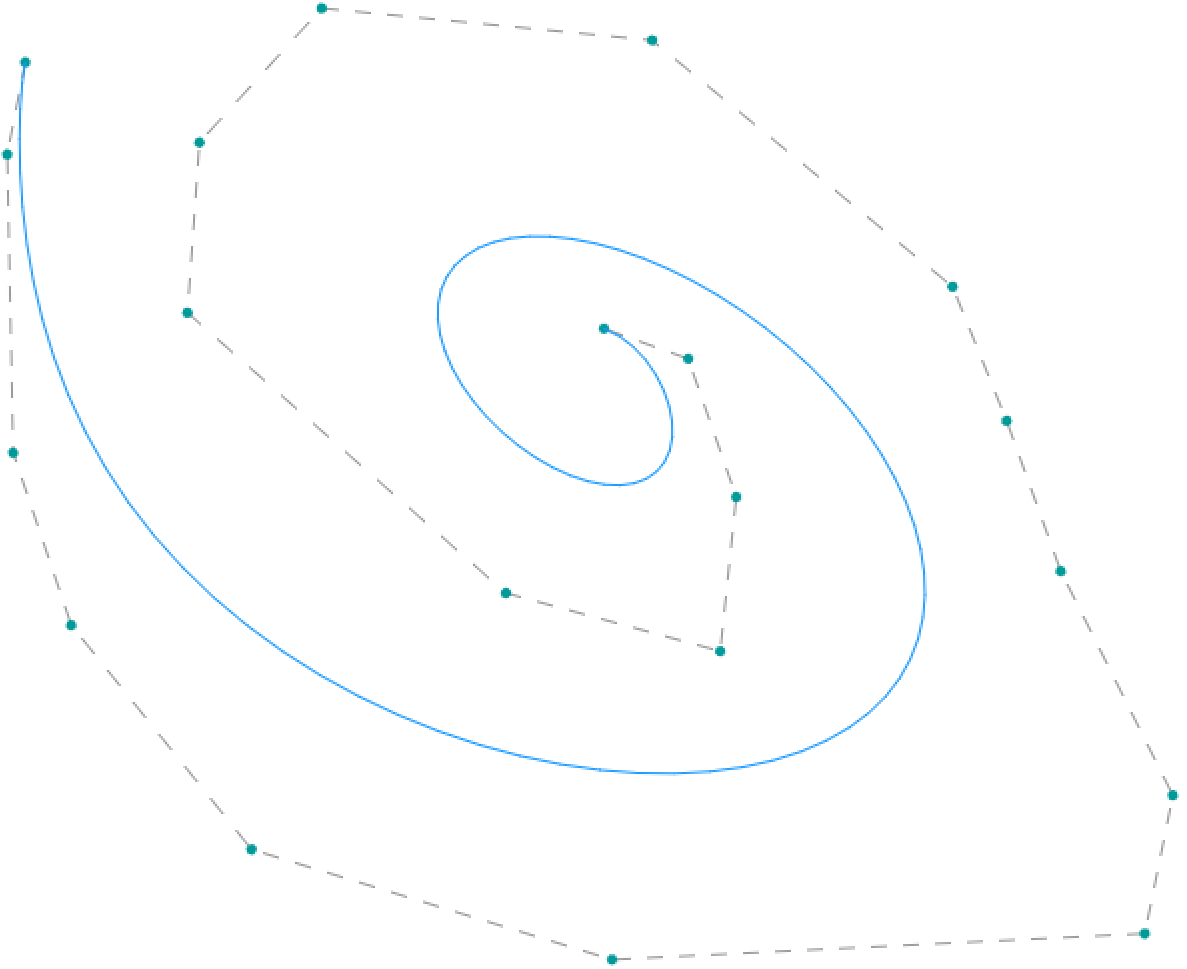
\includegraphics[width=0.7\textwidth]{bezier}
    \caption{Un esempio del risultato\label{fig:bezier}}
    %\vspace{-0.3cm}
\end{figure}

\newpage
\section{Suddivisione Adattiva}
Questo scenario richiama la routine \texttt{drawSubdividedCurve\-(float points[MAX\_CP][3])} che prende un vettore di punti che forma una curva e applica il \textit{flatTest} a tutti i punti interni. Il test si basa sul confronto con un parametro TOL di tolleranza entro cui la curva è considerata \textit{flat} e quindi deve essere disegnata. Se il test è positivo, la curva viene disegnata con un insieme di segmenti che collegano i punti del vettore. Se viceversa il test è negativo, viene suddivisa la curva in due sotto-curve con stesso numero di punti e viene richiamata ricorsivamente la ruotine \texttt{drawBezierCurve}. La suddivisione viene effettuata considerando ciò che si ottiene applicando \textit{De Casteljau} con parametro $t=0.5$. Utilizzando le slide del corso (figura \ref{fig:c1c2}), si può illustrare meglio come è possibile ottenere le due sotto-curve nel caso di una curva iniziale di 4 punti. La parte \textit{gialla} rappresenta la curva iniziale, mentre la parte arancione rappresenta la prima sotto-curva e quella rossa, la seconda.


 \begin{figure}[htb]
    \centering
    \vspace{-0.3cm}
    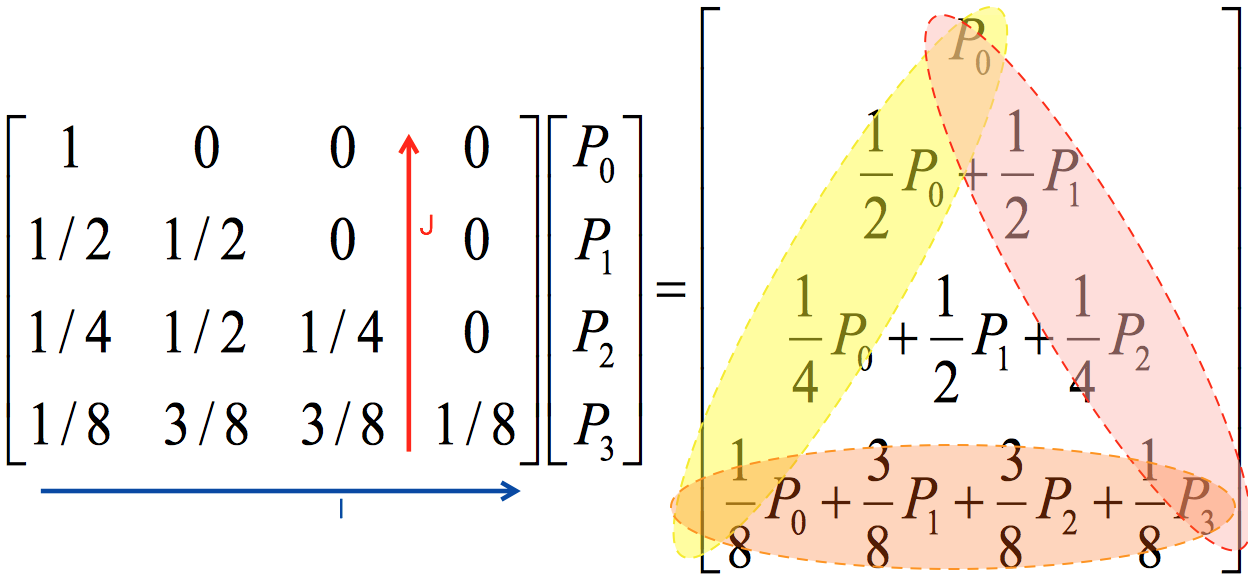
\includegraphics[width=0.6\textwidth]{c1c2}
    \caption{\label{fig:c1c2}}
    \vspace{-0.3cm}
\end{figure}

Un esempio del risultato:
\begin{figure}[hbt]
    \centering
    \subfloat[Con una sola subdivide]{{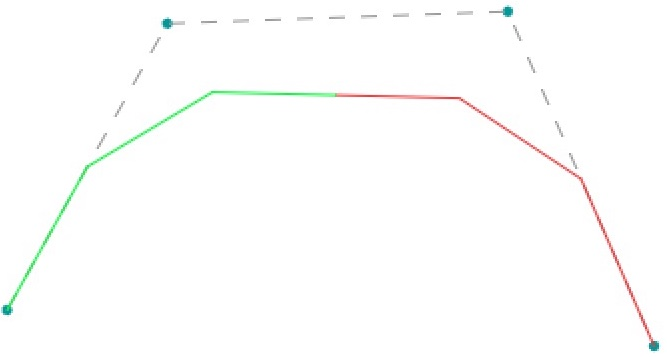
\includegraphics[height=2.8cm]{subdivide} }}%
    \subfloat[Risultato finale]{{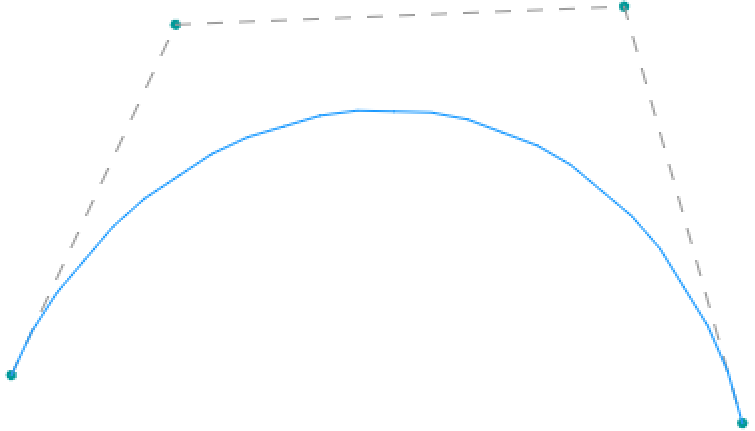
\includegraphics[height=2.8cm]{finalsub} }}%

\end{figure}

\textbf{Nota}: se si utilizza un TOL elevato con questa modalità, in quanto approssimazione, si hanno scarsi risultati quando vi sono pochi punti, mentre quando ve ne sono molti si ha un ottimo riscontro visivo. Ecco un confronto con il normale algoritmo di De Casteljau con un parametro t con precisione $0.01$.

\begin{figure}[hbt]
    \centering
    \subfloat[De Casteljau]{{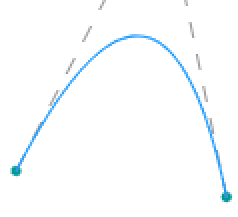
\includegraphics[height=3.5cm]{dec1} }}%
    \subfloat[Subdivision]{{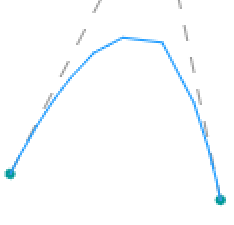
\includegraphics[height=3.5cm]{sub1} }}%
    \subfloat[De Casteljau]{{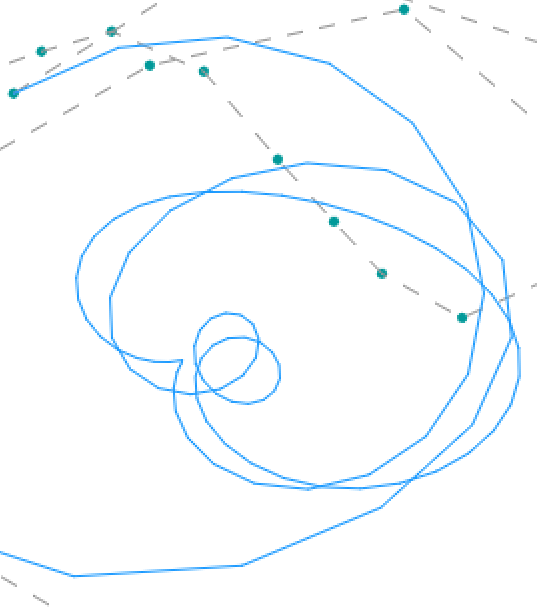
\includegraphics[height=3.5cm]{dec2} }}%
    \subfloat[Subdivision]{{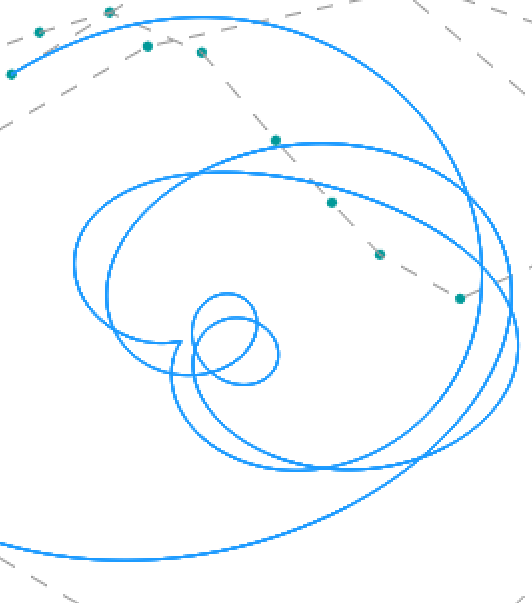
\includegraphics[height=3.5cm]{sub2} }}%
	\vspace{-0.3cm}
\end{figure}

\newpage


\section{Modalità interattiva}
\label{interactive}
Questo scenario permette di disegnare una curva costituita da più curve di Bézier con un grado massimo definito. Questo implica che durante la costruzione del curva vi siano sotto-curve \textit{complete}, ovvero che raggiungono il grado massimo e una sola possibile sotto-curva \textit{in costruzione}, ovvero che ha grado minore al grado massimo. In entrambi i casi viene richiamata la routine \textit{drawBezierCurve}, ma con diversi parametri di ingresso. Per la curva in costruzione, fa uso di:
\begin{itemize}
  \item \textbf{newCurveBegin}: indica l'indice del vettore dei punti di controllo in cui inizia la curva nuova. È ottenuto sottraendo al numero di punti di controllo i \textit{surplusPoints}, ovvero i punti che compongono la curva in costruzione. Questo valore è ottenuto secondo i seguenti calcoli:
		 \begin{lstlisting}
		 	int completedCurves = (numCP - 1) / degree;
			int surplusPoints = (numCP - 1) % (degree * (completedCurves > 0 ? completedCurves : 1)) + 1;
		 \end{lstlisting}
  \item \textbf{tempDegree} definito come \textit{surplusPoints - 1}
\end{itemize}

Per fare in modo di disegnare tutte le curve complete, si ciclano tutti i punti di controllo e si richiama la routine solo se:
\begin{itemize}
  \item vi è almeno una curva completa (\texttt{completedCurves > 0})
  \item il punto corrente non è il primo punto di controllo (\texttt{c!=0})
  \item il punto corrente è un punto di giunzione (\texttt{c\%degree == 0}) 
  \end{itemize}


 Per meglio comprendere il funzionamento di queste espressioni, riporto l'esempio di 9 punti di controllo con grado massimo per curva pari a 3. 
 I valori che si ottengono sono i seguenti:
\begin{itemize}
  \item \textit{completedCurves} = (9 - 1) / 3 = \textbf{2} --> 2 curve complete.
  \item \textit{surplusPoints} = (9 - 1) \% ($3 \times 2$) + 1 = 8 \% 6 + 1 = \textbf{3} --> 3 punti della curva in costruzione. Ricordo che il settimo punto (punto 6 in figura \ref{fig:surplus}) rappresenta un punto di giunzione ed è quindi parte sia della curva completa 2, sia della curva in costruzione;
\end{itemize}

 \begin{figure}[htb]
    \centering
    %\vspace{-0.7cm}
    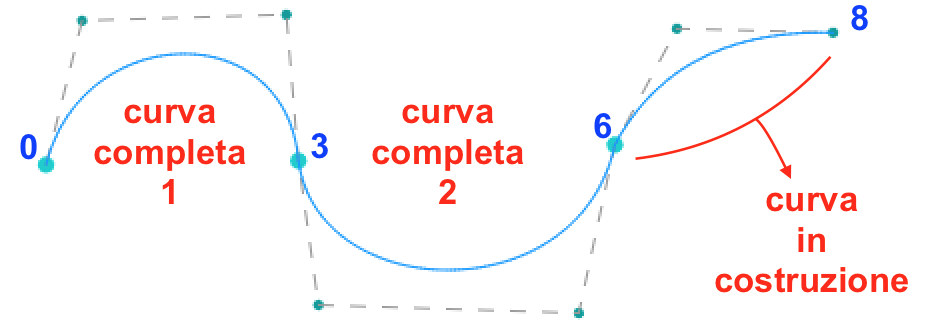
\includegraphics[width=0.8\textwidth]{surplus}
    \caption{\label{fig:surplus}}
    \vspace{-0.3cm}
\end{figure}


\subsection{Modifica della continuità nei punti di giunzione}
Per questo scenario si è scelto di dare la possibilità all'utente di modificare la continuità dei punti di raccordo. È infatti possibile cliccare con il tasto centrale (o click della rotellina) su un punto di raccordo per visualizzare un piccolo menù contenente "$C_0$, $C_1$, $G_1$".

Per creare il menù è stata utilizzata la primitiva \textit{glutCreateMenu()} e sono state aggiunte le 3 voci con \textit{glutAddMenuEntry} e il tasto centrale è stato attaccato tramite la \textit{glutAttachMenu()}. \texttt{changeContinuity(int sel)} è la funzione che a seconda della selezione, applica una posizione diversa al punto successivo al punto di giunzione.

Per poter impostare una diversa continuità in ogni punto di giunzione è necessario tenere in memoria un vettore \textit{junctionContinuity} che viene periodicamente aggiornato nelle funzioni di aggiunta e rimozione dei punti di controllo e in \textit{changeContinuity}.

Nel caso di aggiunta di un punto di controllo successivo ad un punto di raccordo con continuità $C_1$ o $G_1$, è necessario proiettare il punto alla stessa distanza che intercorre tra il punto di raccordo e il punto precedente (nota: per $G_1$ si è scelto di proiettare allo stesso modo di $C_1$, per semplicità). Per fare in modo che il punto sia aggiunto \textit{in continuità}, basta applicare una interpolazione con parametro t = -1 tra il punto di giunzione e il punto precedente e si ottengono le coordinate del nuovo punto.

La funzione peculiare di questo scenario è la \texttt{movePoint()} che viene chiamata ogni volta che l'utente trascina un punto con il tasto destro del mouse. La funzione applica \textbf{sempre} la variazione $\delta$x e $\delta$y sommandole alle coordinate del \textbf{punto selezionato} (ottenuto con la \texttt{highlightPoint()}). Anche questa funzione fa uso delle \textit{completedCurves} e se ve ne è almeno una, distingue i casi in cui il punto che l'utente sta spostando sia un punto che precede o che segue un punto di raccordo. Vi è inoltre la distinzione sulla continuità del punto di giunzione:
\begin{itemize}
  \item se \textbf{il punto selezionato è un punto di giunzione} allora applico le variazioni $\delta$x e $\delta$y anche ai due punti, precedente e successivo.
  \item se \textbf{il punto selezionato PRECEDE un punto di giunzione}, allora si controlla la continuità nel punto di giunzione:
  	\begin{itemize}
  		\item \textbf{$C_1$}: si applica la variazione \textbf{invertita di segno} dello spostamento al punto \textbf{successivo al punto di giunzione}
  		\item \textbf{$G_1$}: si utilizza la funzione \texttt{getRotationPoints(centerPoint)} per ottenere le nuove coordinate del punto \textbf{successivo al punto di giunzione}
  	\end{itemize}
  \item se \textbf{il punto selezionato SEGUE un punto di giunzione}, allora si controlla la continuità nel punto di giunzione e analogamente si applicano nuove coordinate al \textbf{punto precedente al punto di giunzione}.
\end{itemize}


\begin{wrapfigure}{l}{0.3\textwidth} %this figure will be at the right
    \centering
    \vspace{-0.3cm}
    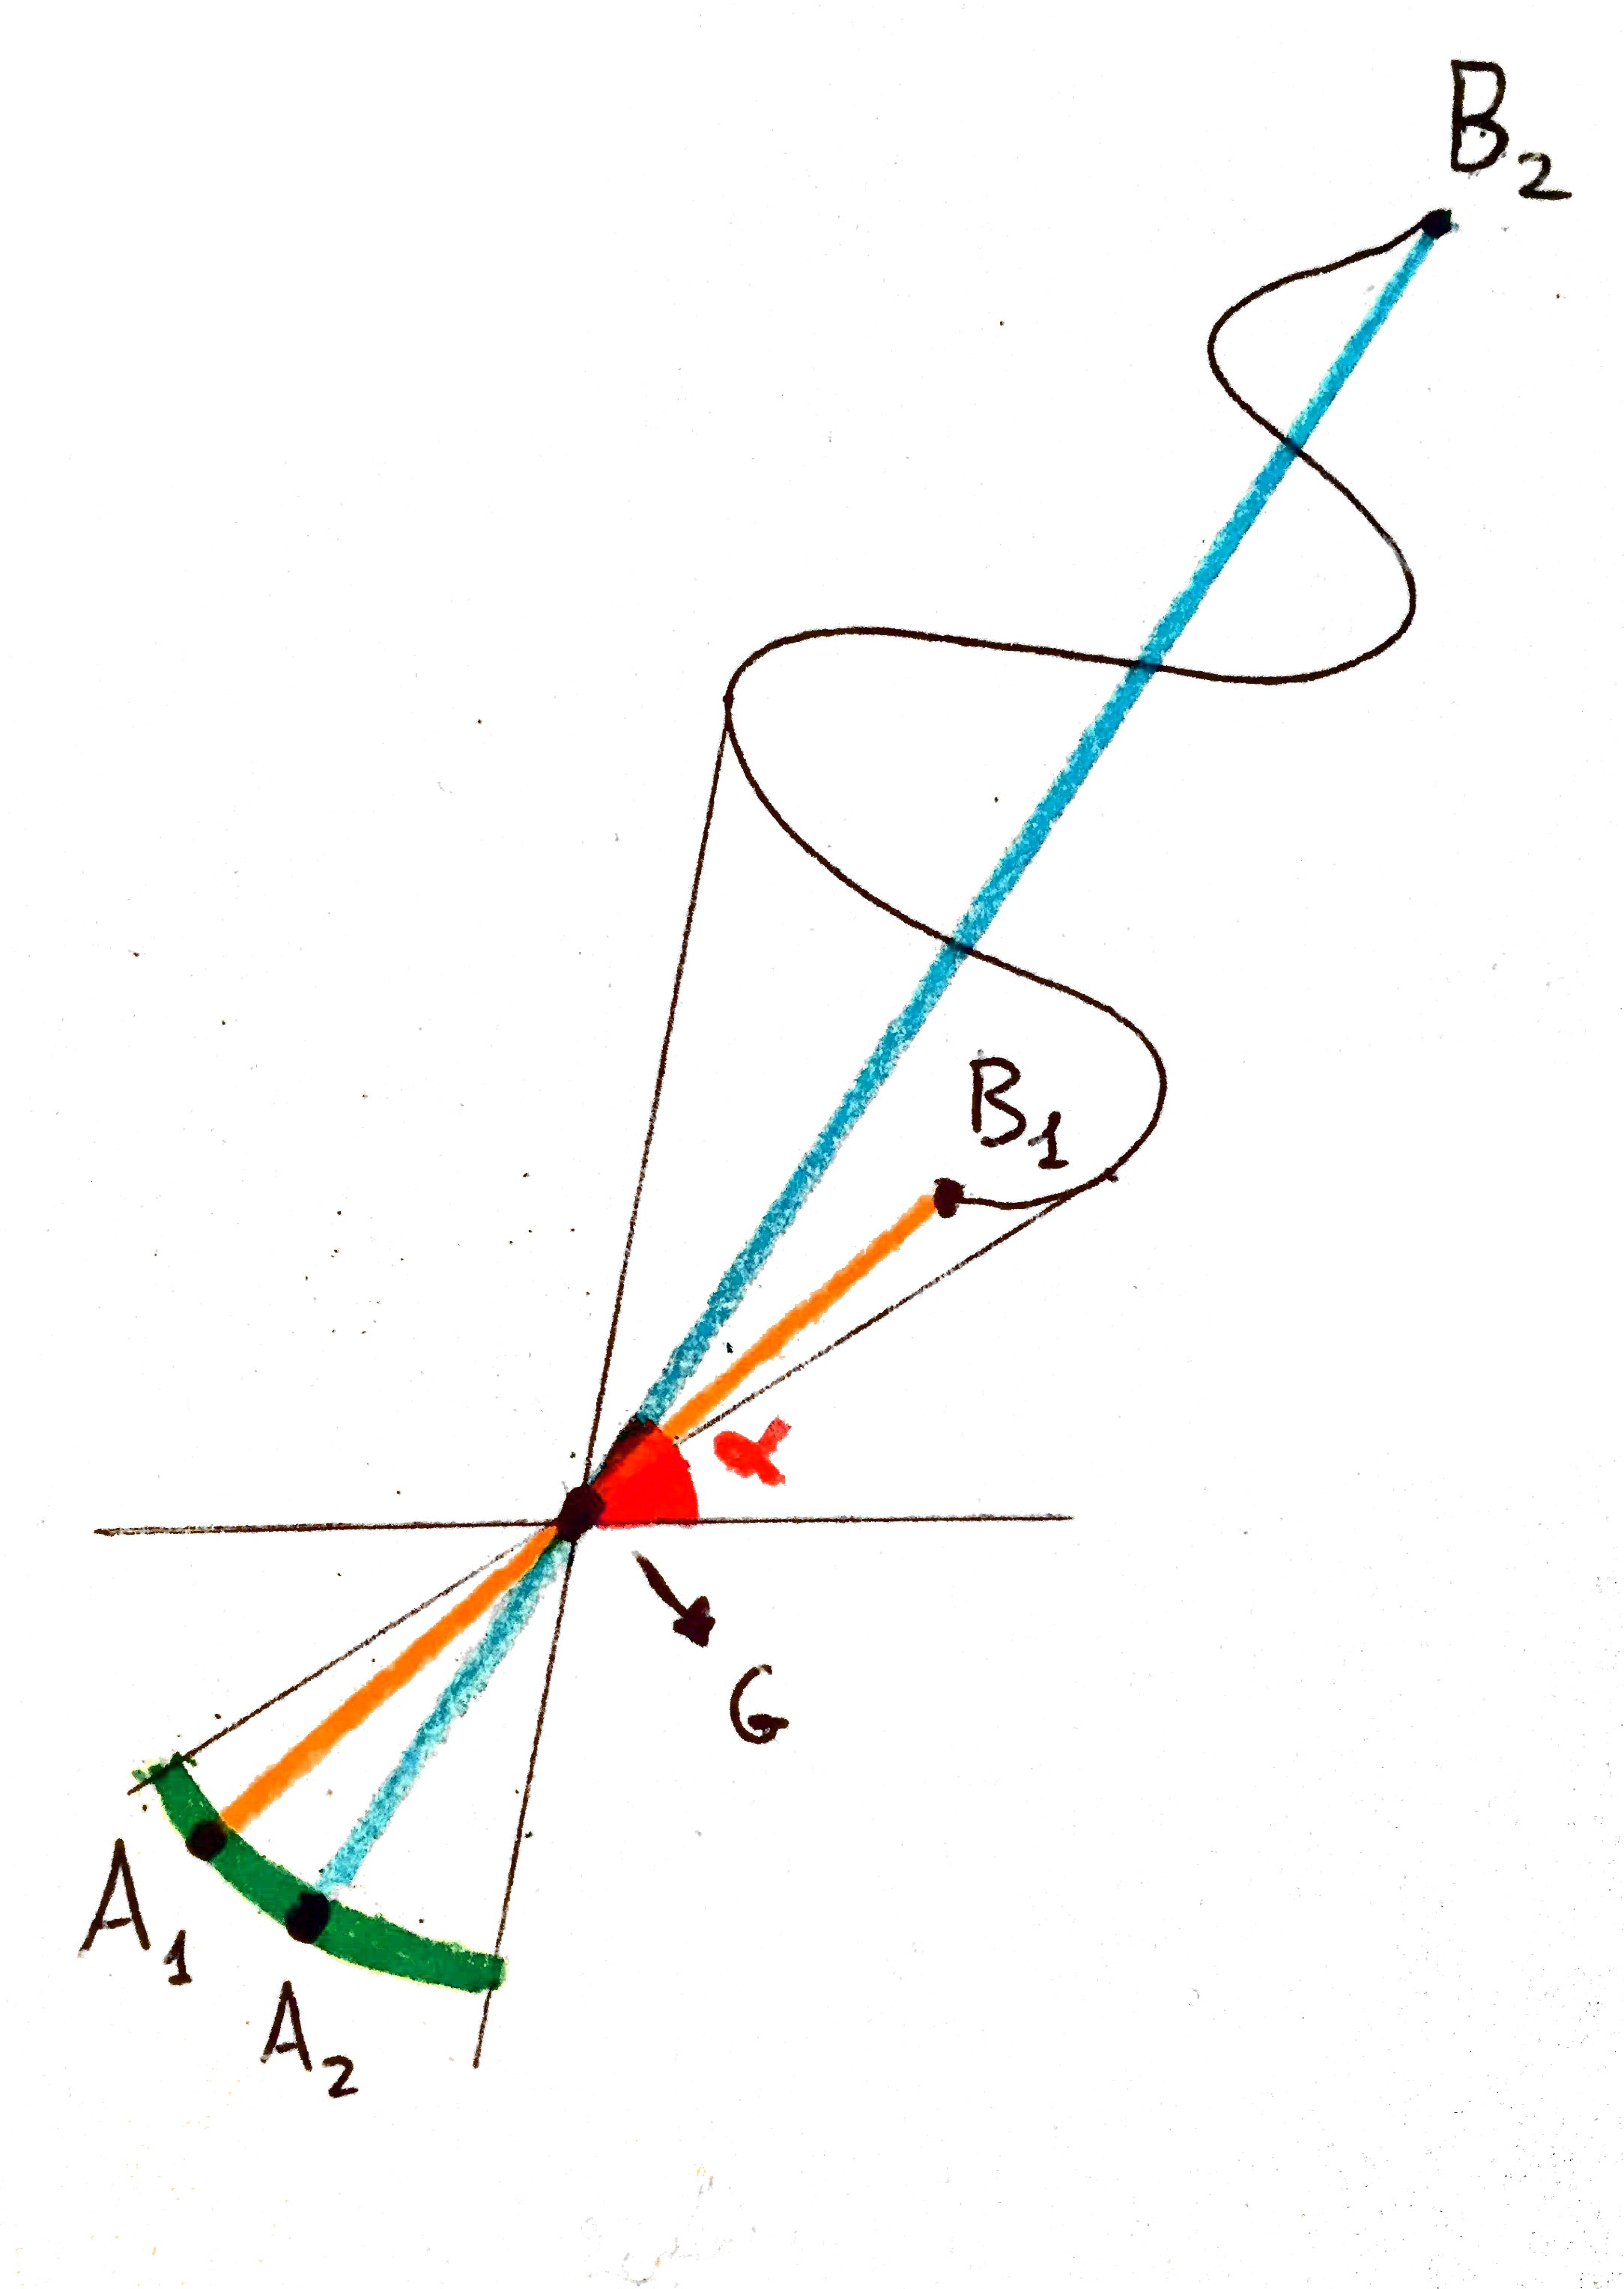
\includegraphics[height=7cm]{rotate}
    \caption{\label{fig:rotate}}
\end{wrapfigure}

\newpage %==============NEWPAGE============%

La funzione \texttt{getRotationPoints(centerPoint)} prende in ingresso l'indice del punto di giunzione attorno a cui dovrà far ruotare il punto opposto al \textit{selectedPoint}. Prendiamo come esempio l'immagine \ref{fig:rotate} per illustrarne il funzionamento.\\

G è il punto di giunzione con continuità $G_1$ e $B_1$ è il punto selezionato. Se lo si trascina nello spazio, il punto $A_1$ dovrà seguirlo mantenendo sempre la distanza dal centro, muovendosi quindi sulla traiettoria circolare verde. Alla prima chiamata, la funzione calcola il raggio di questa traiettoria e lo salva globalmente per non doverlo ricalcolare ad ogni spostamento del punto $B_1$. Ad ogni chiamata, la funzione calcola l'angolo $\alpha$ attraverso la distanza tra G e $B_2$ e lo applica in seno e coseno alle nuove coordinate del punto $A_2$.\\


Il risultato finale è il seguente. Si possono notare i 3 diversi esempi di continuità in 3 diversi punti di giunzione.
 \begin{figure}[htb]
    \centering
    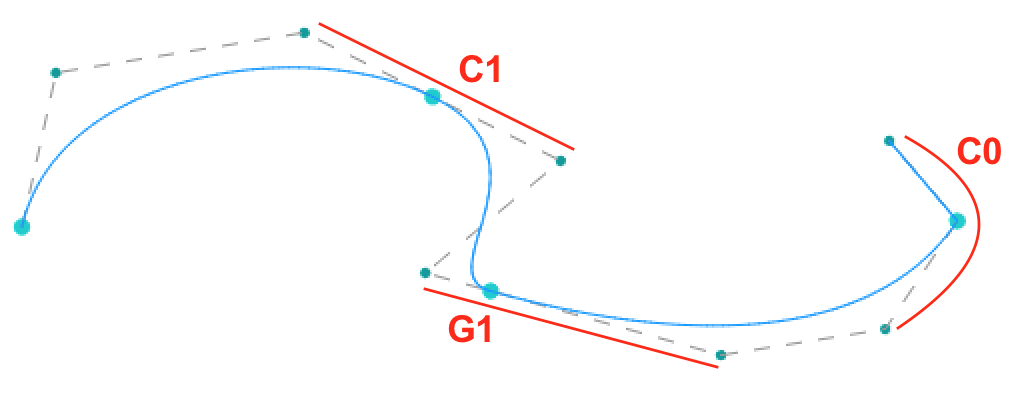
\includegraphics[width=\textwidth]{interactive-result}
    \caption{\label{fig:interactive-result}}
    \vspace{-0.3cm}
\end{figure}




































%